%!TEX root = ../planets-notes.tex

\begin{quote}The true logic of this world is  in the calculus of probabilities. ---James Clerk Maxwell\end{quote}

\newthought{Astronomical observations produce \emph{data}}---sets of numbers from measurements. To advance our understanding of astronomy, we must compare this data to an underlying hypothesis or model.  To make this comparison, we compute some \newterm{statistic} $s$ from the data $\{\mathcal{D}\}$ and assess the likelihood of the value of $s$ given our hypothesis.

As a naive example, we might sum over the differences between the predictions $\prob = \{p_{i}\}$ of a model and the observations $\{D_{i}\}$:
\[ s = \sum_{i} \left(p_{i}-D_{i}\right)^{2}. \]
The data $D_{i}$ could be the transit times for an exoplanet, and $p_{i}$ would be our predicted transit times given a model of the orbit.
In this case, $s=0$ would signify perfect agreement. Nothing is ever perfect, however; what would we make of $s$ being small but non-zero?  We need a figure-of-merit\sidenote{And of course, we want to find the best choice of statistic $s$ for assessing how well the model fits the data.}: given some small value of $s$, is it \emph{likely} that the model is consistent with the data?  If we judge the value of $s$ to be implausible, we say that the model, or hypothesis, is not supported by the data.  

The converse case of $s$ having a value with a high probability does \emph{not}, however, ``rule in'' the hypothesis---at best, the hypothesis is consistent with observations, but other hypotheses may also be consistent. The goal is to amass an ever larger body of evidence supporting the hypothesis, but one can never prove it conclusively.

\section{Basic Rules of Probability and Combinatorics}

Having motivated the problem, we now step back and ask, what is meant by probability? We are familiar with many examples from our everyday experience. What is the probability of drawing an ace from a deck of cards? What is the probability of rain tomorrow? What is the probability that our candidate will win the election?

\begin{exercisebox}[Meaning of ``probability'']
Think of some different situations in which you might use the word ``probability''.  How does the definition of probability differ among these situations?
\end{exercisebox}

It is not immediately obvious that different usages of the term are consistent. To give two examples:

\begin{enumerate}
\item A ``fair'' die is cast; we say that the probability of rolling a $\bullet$ is $\prob(\bullet) = 1/6$.  What does this mean?  We may mean that if we were to roll the die a very large number of times $N$, or roll a large number $N$ of dice, then the number of those tries yielding a $\bullet$ tends toward\sidenote{This definition carries the prior assumption that all sides are equally likely and that $0\leq\prob\leq 1$.}
\[ \prob(\bullet) = \lim_{N\to\infty} \frac{N(\bullet)}{N} = \frac{1}{6}. \]
Note that this is an \emph{assertion}: if we did this experiment and found that $\prob_{\!\mathrm{exp}}(\bullet) \neq 1/6$, we would claim the die is \emph{loaded}!

\item The Newtonian constant of gravitation is
\[ G = \val{\left(6.67384\pm80\right)\ee{-11}}{\meter^{3}\usk\kilo\gram^{-1}\usk\second^{-2}}. \]
What does the ``$\pm80$'' mean? It signifies that the value of $G$ has some specified probability of lying in the interval $6.67304\leq G\times 10^{11} \leq 6.67464$.
This is a different sense of probability than that in the first example: the value of $G$ has a single, definite value, and here the probability reflects the \emph{degree of certainty} we attach to its measured value.
\end{enumerate}

\newthought{To start making this more precise,} let's introduce some terms\cite{Durrett1994The-Essentials-}:
For an experiment or observation there is a set of all possible outcomes, called the 
\newterm{sample space}. A subset of possible outcomes is an \newterm{event}.
We describe our events as subsets of a sample space $\Omega$, as shown in Figure~\ref{f.set-1}.  We write, e.g., $A \subset \Omega$. An impossible event is $\emptyset$, the empty set.  When we say ``not $A$'' we mean $A^{c}$,  the complement of $A$ (shaded region in Fig.~\ref{f.set-2}).
When we say ``$A$ or $B$'' we mean ``$A$ or $B$ or both'' and denote this by $A\cup B$ (Fig.~\ref{f.set-3}).
Finally, when we say ``$A$ and $B$'' we write $A\cap B$ (Fig.~\ref{f.set-4}).  If ``$A$ and $B$ are mutually exclusive'' then we write $A\cap B =\emptyset$ and we say that the sets are 
\newterm{disjoint}, like $A$ and $B$ in Fig.~\ref{f.set-1}.

For example, if we roll two dice, there are $6\times 6 = 36$ possible outcomes. This is our sample space. Suppose we wish to have the sum of our two dice be seven; we'll call this event $A$. There are six such possibilities for event $A$: $\{(1,6),(2,5),(3,4),(4,3),(5,2),(6,1)\}$. Now denote by event $B$ those rolls in which at least one die is a 2 (how many possibilities are there for event $B$?); then $A\cap B = \{(2,5),(5,2)\}$. Suppose event $C$ is rolling a sum of 11, for which there are two possibilities: $\{(5,6),(6,5)\}$. In this case, $C\cap B = \emptyset$.

\begin{exercisebox}[Probability of various draws from a deck of cards]
We have a deck of cards consisting of 4 suits ($\clubsuit$, $\diamondsuit$, $\heartsuit$, $\spadesuit$) with 13 cards per suit (A, 2, 3, 4, 5, 6, 7, 8, 9, 10, J, Q, K).  Suppose we draw one card.  There are $13\times 4=52$ possible outcomes.
\begin{enumerate}
\item How many events draw a $\spadesuit$?
\item How many events draw a $4$?
\item How many events draw a $4\spadesuit$?
\item How many events draw a $4$ or a $\spadesuit$?
\end{enumerate}
\label{ex.card-deck}
\end{exercisebox}

\begin{marginfigure}
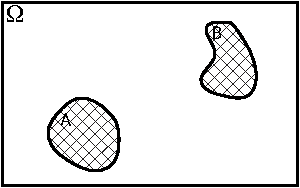
\includegraphics[width=\linewidth]{set-1}
\caption[Sets]{Sets in $\Omega$.}
\label{f.set-1}
\end{marginfigure}
\begin{marginfigure}
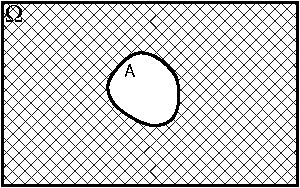
\includegraphics[width=\linewidth]{set-2}
\caption[The complement of a set]{The complement of $A\subset\Omega$.}
\label{f.set-2}
\end{marginfigure}
\begin{marginfigure}
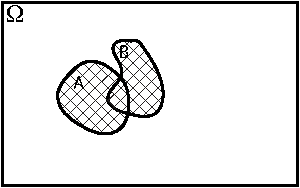
\includegraphics[width=\linewidth]{set-3}
\caption[The union of two sets]{$A\cup B$.}
\label{f.set-3}
\end{marginfigure}
\begin{marginfigure}
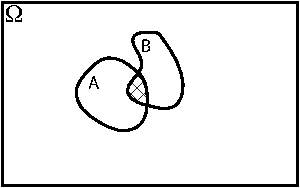
\includegraphics[width=\linewidth]{set-4}
\caption[The intersection of two sets]{$A\cap B$.}
\label{f.set-4}
\end{marginfigure}

\newthought{A probability is a rule} that assigns a number $\prob(A)$ to an event $A$ and obeys the following conditions:
\begin{enumerate}
\item\label{prob.range} $0\le\prob(A) \le 1$
\item\label{prob.complete} $\prob(\Omega) = 1$
\item\label{prob.disjoint} For a set of disjoint (mutually exclusive) events\sidenote[][\baselineskip]{We'll need to be careful when we deal with continuous, rather than discrete, sets.} $\{A_{i}\}$,
\begin{eqnarray*}
 \prob\left(\cup_{i}A_{i}\right) &=& \sum_{i}\prob(A_{i}):\\
 \prob\left(A_{1}\cup A_{2}\cup\ldots\cup A_{N}\right) &=&
 	\prob(A_{1})+\prob(A_{2}) +\ldots+\prob(A_{N}).
\end{eqnarray*}
\item\label{prob.independent} If $A$ and $B$ are independent---meaning that the outcome of $A$ has no influence on the outcome of $B$, and vice versa---then the probability of both events occurring is $\prob(A\cap B) = \prob(A)\prob(B)$.
\end{enumerate}
For an example of independent events, consider drawing a $4\spadesuit$,
\[
 \prob(\textrm{``drawing a 4 and a $\spadesuit$''}) = \prob(4\cap\spadesuit) = \prob(4)\prob(\spadesuit) = \frac{1}{13}\frac{1}{4} = \frac{1}{52}.
 \]
As another example, suppose we roll a die. Each of the possible outcomes are mutually exclusive, so by rules 2 and 3,
\[
	1 = \prob\left(\{1,2,3,4,5,6\}\right) = \prob(1) + \prob(2) +\ldots+\prob(6).
\]
If we assert that all outcomes are equally likely, $\prob(1)=\prob(2)=\ldots=\prob(6)=p$, then $6p = 1$, so $p = 1/6$.

There are a few other properties of sets that are useful to know.
\begin{eqnarray*}
	A\cup B = B\cup A, && A\cap B = B\cap A;\\
	A\cap(B\cap C) = (A\cap B)\cap C, && A\cup(B\cup C) = (A\cup B)\cup C;\\
	A\cap(B\cup C) = (A\cap B)\cup(A\cap C), && A\cup(B\cap C) = (A\cup B)\cap(A\cup C);\\
	A\cup A^{c} = \Omega, && A\cap A^{c} = \emptyset;\\
	\Omega\cap A = A, && \emptyset\cap A = \emptyset.
\end{eqnarray*}
Using these properties and our rules for assigning probabilities, we can deduce a few more formulae. For example, $\prob(A^{c}\cup A) =  \prob(A^{c}) + \prob(A) = \prob(\Omega) = 1$; therefore, $\prob(A^{c}) = 1-\prob(A)$.  Likewise, we can show that $\prob(\emptyset)=0$.  
Finally, we can show that if $A$ and $B$ are not mutually exclusive, but have some overlap, then
\[ \prob(A\cup B) = \prob(A)+\prob(B) - \prob(A\cap B). \]
We encountered an instance of this last rule in exercise~\ref{ex.card-deck}: $\prob(4\cup\spadesuit) = \prob(4)+\prob(\spadesuit) - \prob(4\cap\spadesuit)$.

\begin{exercisebox}[Probability of two events that are not mutually exclusive]
Suppose we draw 1 card from each of 2 decks.  Find the probability that at least one card is an ace, using the following two formulae:
\begin{eqnarray*}
\prob(\textrm{``from deck 1 or from deck 2''}) &=& \prob(\textrm{``from deck 1''})+	\prob(\textrm{``from deck 2''}) \\
&& - \prob(\textrm{``from both deck 1 and deck 2''}).\\
\prob(\textrm{``at least one ace''}) &=& 1-\prob(\textrm{``drawing no ace''}).
\end{eqnarray*}
\end{exercisebox}
 
\newthought{We next need to consider different arrangements of items in a set.} For example, suppose we want to put 5 people in a line. How many ways are there to do this?  For the first spot there are 5 choices.  After assigning this first spot, we move to the second for which there are now 4 choices. Proceeding along in this fashion, the number of possible arrangements is $5\cdot4\cdot3\cdot2\cdot1 \equiv 5!$.\marginnote{The factorial fcn.\ is recursively defined by $m! = m\cdot(m-1)!$, with $0! = 1$, $1! = 1$.}

Suppose we are not picking everything in our set; for example, in a class of 32 we may wish to select just 3 people for different jobs. The number of possibilities is
\begin{equation}\label{e.permutation-class}
 P(32,3) = 32\cdot31\cdot30 = \frac{32\cdot31\cdot30\cdot29\cdot\ldots\cdot 1}{29\cdot\ldots 1} = \frac{32!}{(32-3)!}.
\end{equation}
Here $P(n,k)$ means we are picking $k$ items from a set of $n$ items.

Now suppose we aren't picking individuals for distinct jobs, but just 3 individuals. In this case, the order of how we pick is irrelevant---Autumn, Brook, and Collin is the same as Brook, Collin, and Autumn.  To avoid over-counting different arrangements, we divide $P(32,3)$ from equation~(\ref{e.permutation-class}) by $3!$, giving
\begin{equation}\label{e.combination-class}
\textrm{``32 choose 3''} \equiv {32\choose3} \equiv \mathcal{C}^{32}_{3} = \frac{32!}{(32-3)!3!}.
\end{equation}
More formally, ${n\choose m}$ is the number of ways of choosing $m$ objects from a set of $n$, without regard to order.

One example you may have seen often is the expansion of a binomial.  For example, suppose we wish to expand $(a+b)^{5}$.  There are a total of $2^{5}=32$ terms of the form $a^{5}b^{0}$, $a^{4}b$, $a^{3}b^{2}$, and so on:
\[
	(a+b)^{5} = S_{5}a^{5}+S_{4}a^{4}b+S_{3}a^{3}b^{2}+S_{2}a^{2}b^{3}+S_{1}ab^{4}+S_{0}b^{5}.
\]
For $S_{5}$, there is only one way to get $a^{5}$: we must take one $a$ from each of the terms. As a result, $S_{5}=1$. For $S_{4}$, we pick an $a$ from four of the terms, and a $b$ from the fifth. There are five ways to do this, so $S_{5} =5$. To get $S_{3}$, we must pick an $a$ from 3 of terms.  We don't care about order, so there are ${5\choose3} = 5!/(2!3!) = 5\cdot4\cdot3/(3\cdot2)=10$ ways to do this. Following this line of reasoning, our coefficients are
\begin{center}
\begin{tabular}{rrl}
$m$ & term 			& $S_{m}$\\
\hline
5	& $a^{5}$		& ${5\choose5}=1$\\
4	& $a^{4}b$		& ${5\choose4}=5$\\
3	& $a^{3}b^{2}$	& ${5\choose3}=10$\\
2	& $a^{2}b^{3}$	& ${5\choose2}=10$\\
1	& $a^{1}b^{4}$	& ${5\choose1}=5$\\
0	& $b^{5}$		& ${5\choose0}=1$\\
\end{tabular}
\end{center}
and so
\[ (a+b)^{5} = a^{5}+5a^{4}b+10a^{3}b^{2}+10a^{2}b^{3}+5ab^{4}+b^{5}. \]

These coefficients $n\choose m$ obey several neat recurrence relations. When we are picking our $m$ objects, we have a choice: to pick or not to pick the last item, item number $n$. If we pick the last item, then we must pick the remaining $m-1$ objects from the set $n-1$.  There are ${n-1\choose m-1}$ ways to do so.  If we do not pick the last item, then we must pick all $m$ objects from the set $n-1$. There are ${n-1\choose m}$ ways to do so.  The number of ways for both of these choices must add up to the total number of ways of picking $m$ from $n$:
\begin{equation}\label{e.choose-recurrence}
{n\choose m} = {n-1\choose m-1} + {n-1\choose m}.
\end{equation}
We can make a nice table by putting the coefficients for each $n$ on a row, with $n$ increasing as we go down the table. If $m<0$ or $m>n$ in one of the terms in equation~(\ref{e.choose-recurrence}), we take that term to be 0.  Also, we stagger the entries, so that the terms on the RHS of equation~(\ref{e.choose-recurrence}) are diagonally to the left and right above ${n\choose m}$, like so:
\[ \begin{array}{ccc}{n-1\choose m-1} &  & {n-1\choose m} \\ & {n\choose m} & \end{array}. \]
This gives us the following arrangement, known as \newterm{Pascal's triangle}:
\begin{center}
\begin{tabular}{ccccccccccccc}
	&	&	&	&	&	& 1	&	&	&	&	&	&	\\
	&	&	&	&	& 1	& 	& 1	&	&	&	&	&	\\
	&	&	&	& 1	& 	& 2	& 	& 1	&	&	&	&	\\
 	&	&	& 1	& 	& 3	&	& 3	&	& 1	&	&	&	\\
	&	& 1	&	& 4	&	& 6	&	& 4	& 	& 1	&	&	\\
	& 1	&	& 5	&	& 10&	&10	&	& 5	&	& 1	&	\\
1	&	& 6	&	& 15&	&20	&	&15	&	& 6	&	& 1	\\			
	&	&	&	&	&	&$\ldots$&	&	&	&	& &	\\
\end{tabular}
\end{center}

\begin{exercisebox}[Recurrence relation of Pascal's triangle]
Show that
\[ {n\choose m+1} = {n\choose m} \frac{n-m}{m+1}. \]
Then use this recurrence relation to derive ${6\choose m}, m=1,\ldots 6$, starting from ${6\choose 0} = 1$.
\end{exercisebox}

\newthought{We now have enough machinery to compute the probability of drawing certain hands in poker.} To make this concrete, we insist on no wild cards.  If we draw 5 cards from a deck, there are
\[
{52\choose5} = \frac{52\cdot51\cdot50\cdot49\cdot48}{5\cdot4\cdot3\cdot2\cdot1} = 2\,598\,960 
\]
different possible hands. What is the probability of getting a full house (3 of a kind plus one pair; e.g., 3 eights and 2 kings)? First, there are 13 possibilities for the 3 of a kind: we could have 3 ones, or 3 twos, or 3 jacks, and so on. For our 3 of a kind, there are 4 cards of that type in the deck, and we are selecting 3 of them. After drawing our 3 of a kind, we have 12 choices for the pair. Once we set the type of card for the pair, we then select 2 of the 4 possible cards of that type. The number of such full house combinations is therefore
\[
	13\cdot{4\choose3}\cdot12\cdot{4\choose2} = 13\cdot 4\cdot12\cdot 6 = 3744
\]
and the probability of drawing a full house is therefore $3744/2\,598\,960 = 0.0014$.

What is the probability of getting two pair (e.g., 2 eights, 2 sixes, and a random card)? First, we have to select two types of cards for our pairs. Unlike in the full house, the order is unimportant: 2 eights and 2 sixes is the same as 2 sixes and 2 eights. We therefore choose 2 types of cards out of 13 possible, ${13\choose 2}$, for our pairs. For each pair, we are picking 2 of the 4 possible cards. After doing this, there are 11 possibilities for the remaining card, and for each type there are 4 suits. Thus the number of two pair combinations is
\[
	{13\choose 2}\cdot{4\choose 2}^{2}\cdot11\cdot4 = 123\,552
\]
and the probability of drawing two pair is therefore $123\,552/2\,598\,960 = 0.0475$.

\begin{exercisebox}[Probability of drawing a flush]
What is the probability of drawing a flush (5 cards of the same suit)? To avoid complications, don't worry about whether the combination is a straight flush (cards are in numerical sequence) or a royal flush (cards are A,K,Q,J,10).
\end{exercisebox}

\section{A Probability Distribution: The Random Walk}
We are now ready to tackle a problem that occurs frequently in physics\sidenote{For example, when modeling molecular motion}: the random walk.  Imagine a person who flips a coin before each step---heads to go right, tails to go left.  On average, this person doesn't go anywhere, but from experience you know that sometimes you will get several heads or tails in a row; you wouldn't want to try this random walk if you were a few steps from the edge of a cliff!

We wish to find the probability $\binom{n}{m}{p}$ that after $n$ steps, $m$ will have been to the right and $(n-m)$ to the left, for a net displacement $m-(n-m) = 2m-n$ steps\sidenote{A positive distance means to the right; negative, to the left.}.
To formulate this problem, call the probability to go right $p$; the probability to go left is then $(1-p)$.
Clearly $\binom{n}{m}{p} = 0$ for $m>n$ or $m<0$. Since each step is independent of the others, we can use rule \ref{prob.independent} to obtain the probability for a specific sequence, e.g., RRLRLLRRRL:
\begin{eqnarray}
	\lefteqn{\prob_{n}(RRLRLLRRRL) } \nonumber\\
	&=& p\cdot p\cdot(1-p)\cdot p\cdot(1-p)\cdot(1-p)\cdot p\cdot p\cdot p\cdot(1-p) \nonumber\\
	&=& p^{6}(1-p)^{4}
\label{e.one-sequence},
\end{eqnarray}
since there were 6 steps to the right and 4 to the left. Of course, any sequence of 6 steps to the right and 4 steps to the left has the same probability, so to get the total probability $\prob_{10}(6)$ of having 6 steps out of ten be to the right, we must multiply $p^{6}(1-p)^{4}$ by the number of ways of picking $6$ steps out of $10$ total, which is just $10\choose6$.  More generally, the probability of taking $m$ steps out of $n$ to the right, with each step having a probability $p$ to be to the right, is
\begin{equation}\label{e.binomial}
	\binom{n}{m}{p} = {n\choose m} p^{m}(1-p)^{n-m}.
\end{equation}
This function $\binom{n}{m}{p}$ is called the \newterm{binomial distribution}.

For example, suppose you flip a coin 20 times.  What is the probability of getting exactly 10 heads, assuming even odds for heads:tails?
\[
	\textrm{Answer:}\quad\binom{20}{10}{1/2} = {20\choose10} \left(\frac{1}{2}\right)^{20} = 0.176.
\]
\begin{exercisebox}[Probability distribution for a coin flip]
\label{e.prob-distribution}
Compute $\binom{20}{m}{\frac{1}{2}}$ for $m = 0\ldots20$.  What is the probability of getting 9, 10, or 11 heads?  What is the probability of getting between 7 and 13 heads? \notebook\ \emph{See the accompanying notebook \texttt{binomial.ipynb}.}
\end{exercisebox}

Of course, as the next exercise illustrates, this probability distribution occurs in many contexts, not just in the context of flipping coins or staggering home.

\begin{exercisebox}[Score for random guessing on a multiple-choice exam]
A student takes an exam with 10 multiple choice questions, each with 4 possible responses.  Suppose the student guesses randomly for each question.  What is the probability the student gets 5 or more correct? \notebook\ \emph{See the accompanying notebook \texttt{binomial.ipynb}.}
\end{exercisebox}

\section{Describing the distribution}
\subsection{The mean}

You are probably familiar with taking a simple average of a set of numbers: sum over the set and divide by the number of items in the set.  A related quantity for a probability distribution is the \newterm{mean},
\marginnote{More formally, we can define taking the moment of a distribution with respect to a function $f(x)$ as
\[ \mean{f(x)} = \sum f(x)\prob(x). \]
In general, $\mean{f(x)} \ne f(\mean{x})$.}
\begin{equation}\label{e.mean}
 \mean{m} \equiv \sum_{m=0}^{n} m\binom{n}{m}{p}.
\end{equation}
To show that this behaves as expected, there are some mathematical preliminaries we need to address.  First, let's demonstrate that $\sum\binom{n}{m}{p} = 1$.  The easiest way to show this is to take a concrete example, say $n=5$.  Then
\begin{eqnarray*} \sum_{m=0}^{5}\binom{5}{m}{p} &=& \sum_{m=0}^{5}{5\choose m}p^{m}(1-p)^{n-m}\\
	&=&	p^{5}+5p^{4}(1-p)+10p^{3}(1-p)^{2}+10p^{2}(1-p)^{3}\\
	&& +5p(1-p)^{4}+(1-p)^{5}.
\end{eqnarray*}
Look familiar?  You should convince yourself that this is the binomial
\[ \sum_{m=0}^{5}\binom{5}{m}{p} = \left.\left(p+q\right)^{5}\right|_{q=1-p}
	= \left[p + \left(1-p\right)\right]^{5} = 1. \]
We can use this identity, $\sum\binom{n}{m}{p}=\sum{n\choose m}p^{m}q^{n-m} = (p+q)^{n}$ with $q=1-p$, to help us evaluate various sums over the distribution.

To evaluate the mean, we first notice that each term in the sum of equation~(\ref{e.mean}) can be written $m\binom{n}{m}{p} = {n\choose m} m p^{m} q^{n-m}$.  Now $q = 1-p$; but if we temporarily let $q$ and $p$ vary independently, we can write
\marginnote{By $\partial f/\partial x$, we mean, ``the derivative of $f$ with respect to $x$, holding other variables fixed.''  For example, if $f = f(x,y) = x^{2}y e^{y}$, then $\partial f/\partial x = 2xye^{y}$ and $\partial f/\partial y = x^{2}(1+y)e^{y}$.  Sometimes we write $(\partial f/\partial x)_{y}$ just to make it clear we are holding $y$ fixed.}
\[ 
	m\binom{n}{m}{p} = {n\choose m}p\left(\dd{}{p}\right)_{\!q} p^{m}q^{n-m}
	= p\left(\dd{}{p}\right)_{\!q}\left[{n\choose m}p^{m}q^{n-m}\right].
\]
Hence, the mean is
\begin{eqnarray}
	\mean{m} &=& \sum_{m=0}^{n}m\binom{n}{m}{p} \nonumber\\
	&=& \left[p\left(\dd{}{p}\right)_{\!q}\sum_{m=0}^{n}{n\choose m}p^{m}q^{n-m}\right]_{q=1-p}\nonumber\\
	&=& \left[p\left(\dd{}{p}\right)_{\!q}\left(p+q\right)^{n}\right]_{q=1-p}\nonumber\\
	&=& \left[pn\left(p+q\right)^{n-1}\right]_{q=1-p} = np.
\end{eqnarray}
This makes sense: if we flip a fair coin $n$ times, we expect the average number of heads to be $n/2$.  Notice also that for this distribution the mean is the value for which the probability is highest.

\subsection{The standard deviation}
Although the mean $\mean{m} = np$ gives the most likely value, you know from exercise~\ref{e.prob-distribution} that there is a substantial probability of getting values other than $\mean{m}$. What we want to develop is a measure for how tightly the distribution is clustered about the mean.  We might want something like $\mean{m-\mean{m}}$---that is, what is the average difference from the mean---but this won't do: from the definition of the mean,
\[ \mean{m-\mean{m}} = \mean{m}-\mean{m} = 0. \]
\marginnote{%
From the definition of the mean,
\begin{eqnarray*}
\mean{a+bx} &=& \sum\left[\left(a+bx\right)\prob(x)\right] \\
	&=& a\sum\prob(x) + b \sum x\prob(x)\\
	&=& a+b\mean{x},
\end{eqnarray*}
since $\sum\prob(x)=1$.
}
We could choose something like $\mean{\left|m-\mean{m}\right|}$, which gives a positive-definite measure of the width; a more convenient measurement, however, is the root-mean-square (rms) width $\sqrt{\mean{(m-\mean{m})^{2}}}$.  To calculate this, let's first expand the square:
\[
	\mean{\left(m-\mean{m}\right)^{2}} = \mean{m^{2} - 2m\mean{m} + \mean{m}^{2}}
		= \mean{m^{2}} - \mean{m}^{2}.
\]
To calculate $\mean{m^{2}}$ for the binomial distribution, we use a similar trick from the calculation of $\mean{m}$:
\[
	m^{2}\binom{n}{m}{p} = p\left(\dd{}{p}\right)_{\!q}\left\{ p\left(\dd{}{p}\right)_{\!q} 
	\left[{n\choose m} p^{m}q^{n-m}\right]\right\}.
\]
Therefore
\begin{eqnarray*}
	\mean{m^{2}} &=& \sum_{m=0}^{n}m^{2}\binom{n}{m}{p} \\
	&=& \left\{p\left(\dd{}{p}\right)_{\!q}\left[p\left(\dd{}{p}\right)_{\!q}\sum_{m=0}^{n}{n\choose m}p^{m}q^{n-m}\right]\right\}_{q=1-p} \\
	&=& \left\{p\left(\dd{}{p}\right)_{\!q}\left[p\left(\dd{}{p}\right)_{\!p}\left(p+q\right)^{n}\right]\right\}_{q=1-p} \\
	&=& p\left(\dd{}{p}\right)_{\!q}\left[pn\left(p+q\right)^{n-1}\right]_{q=1-p} \\
	&=& np + n(n-1)p^{2}.
\end{eqnarray*}
Our expression for the rms width is therefore
\begin{eqnarray}
	\left[\mean{\left(m-\mean{m}\right)^{2}}\right]^{1/2} &=& \left[ np + (np)^{2}-np^{2} - (np)^{2}\right]^{1/2}\nonumber\\
	 &=& \left[np(1-p)\right]^{1/2}.
\end{eqnarray}
Notice that although the width of the distribution increases with $n$, the ratio of the width to the average value decreases, $\textrm{width}/\textrm{mean} \propto 1/\sqrt{n}$.  Thus the relative size of fluctuations about the mean decreases as $n$ becomes larger.

\section{The Poisson distribution}

A common limiting case is to have a very small $p$ and a very large $n$. For example, suppose we are receiving X-rays from a dim source with a photon countrate $\val{36}{\hour^{-1}}$; that is, in one hour we receive on average just 36 photons.  In any given second the probability of receiving a photon is $\val{36}{\hour^{-1}}\times \val{1}{\hour}/\val{3600}{\second}\times \val{1}{\second} = 0.01$.  If we point our detector at the source for $\val{500}{\second}$, however, we can expect to receive on average $\lambda = \val{500}{\second}\times\val{0.01}{\second^{-1}} = 5$ photons.

\begin{marginfigure}
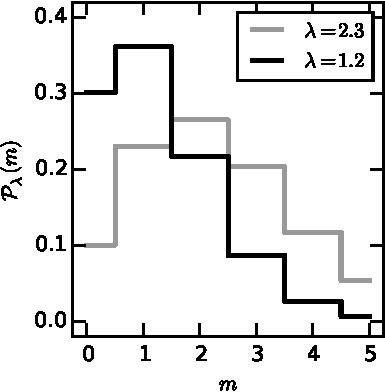
\includegraphics[width=\linewidth]{Poisson}
\caption[The Poisson distribution ]{The Poisson distribution for $\lambda=2.3$ (thick gray lines) and $\lambda=1.2$ (thin black lines).}
\label{f.Poisson}
\end{marginfigure}

Let's take the binomial distribution, eq.~(\ref{e.binomial}), in the limit of $p\ll 1$ while holding $Np=\lambda=\mathrm{const.}$, so that $N = \lambda/p \gg 1$:
\begin{eqnarray*}
	\lefteqn{\lim_{p\to 0,Np\to\lambda}\binom{n}{m}{p}}\\
	 &=& \lim_{p\to 0,Np\to\lambda} \frac{N!}{(N-m)!m!} p^{m} (1-p)^{N-m}\\
	&=& \lim_{p\to 0,Np\to\lambda} \frac{\overbrace{N(N-1)\ldots(N-m+1)}^{\textrm{$m$ terms}}}{m!}p^{m}\frac{(1-\lambda/N)^{N}}{(1-p)^{m}}\\
	&=& \lim_{p\to 0,Np\to\lambda} \frac{(Np)^{m}}{m!}\left[\left(1-\frac{1}{N}\right)\ldots\left(1-\frac{m-1}{N}\right)\right]\frac{(1-\lambda/N)^{N}}{(1-p)^{m}}\\
	&=& \frac{\lambda^{m}}{m!}\lim_{N\to\infty}\left(1-\frac{\lambda}{N}\right)^{N}.
\end{eqnarray*}
Recognizing that the last term is just $e^{-\lambda}$, we obtain the \newterm{Poisson distribution}:
\begin{equation}\label{e.Poisson}
	\prob(m,\lambda) = \frac{\lambda^{m}}{m!}e^{-\lambda}.
\end{equation}
Thus in our example, if we have an average photon countrate of $\val{36}{\hour^{-1}} = \val{0.01}{\second^{-1}}$ and we stare at our source for $\val{500}{\second}$, then $\lambda = 5$ is our expected number of photons, and $\prob(3,\lambda)$ would be the probability of receiving 3 photons in that time.

Not surprisingly, the mean number of events $\mean{m}$ is
\begin{eqnarray*}
	\mean{m} &=& \sum_{m=0}^{\infty} m \frac{\lambda^{m}}{m!}e^{-\lambda}\\
		&=& e^{-\lambda} \lambda \DD{}{\lambda}\sum_{m=0}^{\infty} \frac{\lambda^{m}}{m!}\\
		&=& \lambda.
\end{eqnarray*}
\marginnote[-3\baselineskip]{Recall the expansion
\[ e^{\lambda} = \sum_{m=0}^{\infty}\frac{\lambda^{m}}{m!}. \]
}
The standard deviation is
\begin{eqnarray*}
	\sigma = \sqrt{\mean{\left(m-\mean{m}\right)^{2}}} = \sqrt{\mean{m^{2}}-\mean{m}^{2}}
		&=& \left[e^{-\lambda}\left(\lambda\DD{}{\lambda}\right)^{2}\sum_{m=0}^{\infty}\frac{\lambda^{m}}{m!}-\lambda^{2}\right]^{1/2}\\
		&=& \left[e^{-\lambda}\lambda\DD{}{\lambda}\left(\lambda e^{\lambda}\right)-\lambda^{2}\right]^{1/2}\\
		&=& \sqrt{\lambda}
\end{eqnarray*}
As with the normal distribution, the ratio of width to mean, $\sigma/\mean{m} = 1/\sqrt{\lambda}$, decreases as the mean number of events increases.  

\begin{exercisebox}[Probability of matching birthdays]
A high school graduating class has 400 students.  What is the probability that 2 people in that class have a birthday on January 1?  What about 3 students?
\end{exercisebox}

\begin{exercisebox}
\notebook\ For a photon countrate of $\val{0.01}{\second^{-1}}$, how many seconds of observation are required so that the mean number of photons received is more than $3\sigma$ greater than $0$? The notebook \texttt{signal-to-noise.ipynb} explores the extraction of a weak signal from a noisy background in more detail.
\end{exercisebox}

A historical example of a Poisson distribution is from WWII, when London was targeted by V-1 flying bombs.  A total of 537 V-1 bombs hit London.  To look at where the bombs hit, \citetalt{clarke1946} divided London into 576 districts, each of $\val{0.25}{\kilo\meter^{2}}$ area.  The distribution of bomb strikes went as follows.
\begin{center}
\begin{tabular}{r|rrrrrr}
no.\ bombs & 0 & 1 & 2 & 3 & 4 & $>5$\\
\hline
no.\ districts & 229 & 211 & 93 & 35 & 7 & 1\\
\end{tabular}
\end{center}
That is, 229 districts were unscathed, 211 districts were hit once, and so on, with one unfortunate district being hit by 7 bombs.  Question: were certain districts of London deliberately targeted? Suppose instead that the bombs were just launched in the general direction of London and fell randomly over the area.  In that case, the probability of a district being hit by any one bomb is small---$1/576$ to be exact.  The average number of bombs per district is $\lambda = 537/576 = 0.9323$, so we would expect a Poisson distribution if the bombs were distributed randomly, with the expected number of districts hit by $m$ bombs as follows.
\[ \mathcal{N}(m) = 576\times \prob_{\lambda}(m) = 576\times \frac{\lambda^{m}}{m!}e^{-\lambda}, \]
\begin{center}
\begin{tabular}{r|rrrrrr}
$m$ & 0 & 1 & 2 & 3 & 4 & 5\\
\hline
$\prob_{\lambda}(m)$ & 0.3937 & 0.3670 & 0.1711 & 0.0532 & 0.0124 & 0.0023\\
$\mathcal{N}(m)$ & 227 & 211 & 99 & 31 & 7 & 1
\end{tabular}
\end{center}
This matches the observed distribution well, and the pattern of hits is therefore consistent with the bombs being scattered randomly over the London area.\sidenote{This was probably small consolation to the residents of the districts hit multiple times.}

\section{An alternate derivation of the Poisson distribution}
\marginnote{This section is not essential and can be omitted}
The Poisson distribution is frequently encountered when observing in X- or $\gamma$-rays: the probability of receiving a single photon in any given second is small, but over a long period of time (several thousands of seconds, e.g.) there will be a sizable number of photons collected.  What is the probability of receiving $N$ photons in a given time interval? In this case, we can derive the Poisson distribution independently from the binomial distribution.

To do so, assume that our time intervals $\dif t$ are sufficiently short that the chance of receiving more than one photon in $\dif t$ is negligible.  Then in $\dif t$ we either receive one photon with probability $\mu\dif t \ll 1$ or we receive no photons with probability $(1-\mu)\dif t$.  Let us take $\mu$ to be a constant, and assume that non-overlapping intervals of time are statistically independent---that is, the chance of receiving a photon in a given interval doesn't depend on what happened in the previous interval.  Then there are two ways to receive $N$ photons in a time $t+\dif t$: we can receive $N$ photons in a time $t$ and no photons in the interval $(t,t+\dif t)$; or we can receive $N-1$ photons in a time $t$ and one photon in the interval $(t,t+\dif t)$.  The probability of receiving $N$ photons in a time $t+\dif t$ is the sum of the probabilities of these two scenarios:
\[
	\prob_{\mu}(N;t+\dif t) = (1-\mu\dif t)\prob_{\mu}(N;t) + \mu\dif t \prob_{\mu}(N-1;t).
\]
Rearranging terms and taking the limit $\dif t \to 0$ gives us a differential equation,
\begin{eqnarray}
\DD{\prob_{\mu}(N;t)}{t} &=& \lim_{\dif t\to 0} \frac{\prob_{\mu}(N;t+\dif t)-\prob_{\mu}(N;t)}{\dif t} \nonumber\\
&=& \mu\left[\prob_{\mu}(N-1;t)-\prob_{\mu}(N;t)\right].
\label{e.poisson-recursion}
\end{eqnarray}
The probability of getting no events in $t+\dif t$ is
\[ \prob_{\mu}(N=0;t+\dif t) = (1-\mu\dif t)\prob_{\mu}(N=0;t), \]
which gives the differential equation
\[ \DD{\prob_{\mu}(0;t)}{t} = -\mu\prob_{\mu}(0;t) \]
with solution $\prob_{\mu}(N=0;t) = e^{-\mu t}$.  We fix the constant of integration by setting $\prob_{\mu}(N=0;t=0) = 1$.

Now that we have $\prob_{\mu}(N=0;t) = e^{-\mu t}$, we can solve the differential equation~(\ref{e.poisson-recursion}) for $\prob_{\mu}(N=1;t)$,
\[ \DD{\prob_{\mu}(N=1;t)}{t} = \mu\left[e^{-\mu t} - \prob_{\mu}(N=1;t)\right], \]
with solution $\prob_{\mu}(N=1;t) = (\mu t)e^{-\mu t}$, as you can verify.  We can then find a solution for $\prob_{\mu}(N=2;t)$; and continue in that fashion to find the Poisson distribution:
\begin{equation}\label{e.Poisson-alt}
	\prob_{\mu}(N;t) = \frac{\lambda^{N}}{N!} e^{-\lambda}
\end{equation}
with $\lambda=\mu t$.

\begin{exercisebox}[Recurrence relations for the Poisson distribution]
Show that $\prob_{\mu}(N;t)$ (eq.~[\ref{e.Poisson-alt}]) satisfies the recursion relation, equation~(\ref{e.poisson-recursion}). Since $\prob_{\mu}(N=1;t)$ also satisfies the equation, this proves via induction that equation~(\ref{e.Poisson-alt}) is the correct distribution.
\end{exercisebox}

\section{The normal, or Gaussian, distribution}

To motivate our discussion of the probability distribution for a continuous variable, suppose we wish to find the average location of a person doing the random walk.  If all the steps have the same unit length, then for $m$ steps to the right the position is $x = m - (n-m) = 2m-n$ with mean value $\mean{x} = 2\mean{m}-n$.  Now suppose that the steps are not all of the same length, but instead have some random distribution with mean length $\mean{\ell}$. We'd like to know the probability, $\prob_{n}(x)$, of our walker being at  position $x$.

\newthought{The first conceptual hurdle we reach} is that it makes no sense to ask: ``What is the probability $\prob_{n}(x)$ of the walker being at \emph{exactly} $x=0.2914578329$?'' There are an innumerable infinity of real numbers, so the probability of hitting any particular real number exactly is vanishingly small.  What we instead must ask is, ``What is the probability $\prob_{n}(x;\Delta x) = p(x)\Delta x$ of being in some interval $\Delta x$ about $x$''?  We call $p(x)$ the \newterm{probability density} or \newterm{probability distribution} and assume that $\prob(x) \propto \Delta x$ for sufficiently small $\Delta x$.

Although the formal proof is beyond the scope of the course, it can be shown that in the limit of large $N$,
\begin{equation}\label{e.gaussian}
p(x; \mu,\sigma) = \frac{1}{\sqrt{2\pi}\sigma} \exp\left[-\frac{\left(x-\mu\right)^{2}}{2\sigma^{2}}\right];
\end{equation}
for this random walk with steps of average length $\mean{s}$, $\mu = (2\mean{m}-n)\mean{s}$ and $\sigma  \propto \sqrt{n}\mean{s}$.  This distribution is known as the \newterm{normal}, or \newterm{Gaussian}, probability distribution.  The factor $1/(\sqrt{2\pi}\sigma)$ ensures that the probability has the correct normalization,
\marginnote{Recall that
\[ \int_{-\infty}^{\infty} e^{-\beta x^{2}}\,\dif x = \sqrt{\frac{\pi}{\beta}}.\]
}
\[ \int_{-\infty}^{\infty}p(x;\mu,\sigma)\,\dif x = 1. \]
The peak, or most probable value, of this distribution is at $x=\mu$.

We can verify that the mean of the normal distribution is $\mu$: letting $z = x-\mu$,
\begin{eqnarray*}
\lefteqn{\int_{-\infty}^{\infty} \frac{x}{\sqrt{2\pi}\sigma} \exp\left[-\frac{\left(x-\mu\right)^{2}}{2\sigma^{2}}\right] \,\dif x = }  \\
	&& \int_{-\infty}^{\infty} \frac{z}{\sqrt{2\pi}\sigma} \exp\left[-\frac{z^{2}}{2\sigma^{2}}\right] \,\dif z + \int_{-\infty}^{\infty} \frac{\mu}{\sqrt{2\pi}\sigma} \exp\left[-\frac{z^{2}}{2\sigma^{2}}\right] \,\dif z 
\end{eqnarray*}
The first term on the RHS vanishes because it is odd in $z$; that is,
\[ 
	\int_{-\infty}^{0} \frac{z}{\sqrt{2\pi}\sigma} \exp\left[-\frac{z^{2}}{2\sigma^{2}}\right] \,\dif z = -\int_{0}^{\infty} \frac{z}{\sqrt{2\pi}\sigma} \exp\left[-\frac{z^{2}}{2\sigma^{2}}\right] \,\dif z.
\]
The second term is just $\mu \int_{-\infty}^{\infty} p(z)\,\dif z = \mu$.


\begin{marginfigure}
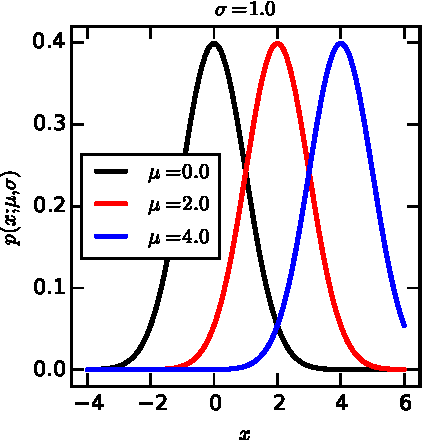
\includegraphics[width=\linewidth]{Normal_sigma1}
\caption[Normal distributions with different means]{Normal, or Gaussian, probability distribution for different values of $\mu$ with $\sigma=1$.}
\label{f.Normal-vary-mu}
\end{marginfigure}

To compute the standard deviation, $\sqrt{\mean{(x-\mean{x})^{2}}} = \sqrt{\mean{x^{2}}-\mean{x}^{2}}$, 
we use the following trick:
\[
	\int_{-\infty}^{\infty}x^{2}e^{-\beta x^{2}}\,\dif x 
		= -\dd{}{\beta}\int_{-\infty}^{\infty}e^{-\beta x^{2}}\,\dif x = -\dd{}{\beta}\sqrt{\frac{\pi}{\beta}} = \frac{1}{2}\frac{\sqrt{\pi}}{\beta^{3/2}}.
\]
To use this, we first change variables to $z = x-\mu$; then
\begin{eqnarray*}
	\mean{x^{2}} - \mean{x}^{2} &=& \int_{-\infty}^{\infty}\frac{z^{2}+2z\mu+\mu^{2}}{\sqrt{2\pi}\sigma} \exp\left[-\frac{z^{2}}{2\sigma^{2}}\right]\,\dif z - \mu^{2}\\
		&=& \int_{-\infty}^{\infty}\frac{z^{2}}{\sqrt{2\pi}\sigma} \exp\left[-\frac{z^{2}}{2\sigma^{2}}\right]\,\dif z + 2\mu \int_{-\infty}^{\infty}\frac{z}{\sqrt{2\pi}\sigma} \exp\left[-\frac{z}{2\sigma^{2}}\right]\,\dif z \\
		&& + \mu^{2}\left\{ \int_{-\infty}^{\infty} \frac{1}{\sqrt{2\pi}\sigma} \exp\left[-\frac{z}{2\sigma^{2}}\right]\,\dif z - 1\right\}.
\end{eqnarray*}

\noindent You should convince yourself that the last term (in $\{\,\}$) is zero; also, the middle term vanishes because it is odd in $z$.  We then use our trick to evaluate the first term and obtain,
\begin{eqnarray*}
	\mean{x^{2}} - \mean{x}^{2} &=& \int_{-\infty}^{\infty}\frac{z^{2}}{\sqrt{2\pi}\sigma} \exp\left[-\frac{z^{2}}{2\sigma^{2}}\right]\,\dif z \\
	&=& \frac{\sqrt{\pi}}{2}(2\sigma^{2})^{3/2}\frac{1}{\sqrt{2\pi}\sigma} = \sigma^{2}.
\end{eqnarray*}
Plots of the normal distribution for different values of $\sigma$ and $\mu=0$ are shown in Figure~\ref{f.Normal-vary-sigma}.
\begin{quote}
\notebook\ The notebook \texttt{mean-standard-deviation.ipynb} explores the properties of the normal distribution in more detail.
\end{quote}

\begin{marginfigure}
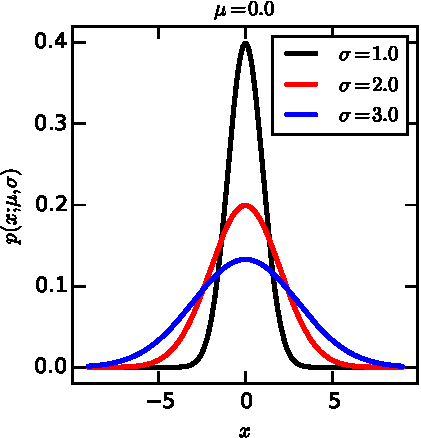
\includegraphics[width=\linewidth]{Normal_mu0}
\caption[Normal distributions with different standard deviations]{Normal distribution for $\mu=0$ and varying values of $\sigma$.}
\label{f.Normal-vary-sigma}
\end{marginfigure}

\section{The cumulative probability distribution}

Now that we have our probability distribution, we can ask questions such as, ``For a mean value $\mu$ and standard deviation $\sigma$, what is the probability that $a < x < b$?'' or ``What is the probability that $x < c$?''

To answer questions like these, we integrate $p$ over the range of interest:
\begin{eqnarray*}
	\prob(a< x < b) &=& \int_{a}^{b} \frac{1}{\sqrt{2\pi}\sigma}\exp\left[-\frac{(x-\mu)^{2}}{2\sigma^{2}}\right]\,\dif x,\\
	\prob(x < c) &=& \int_{-\infty}^{c} \frac{1}{\sqrt{2\pi}\sigma}\exp\left[-\frac{(x-\mu)^{2}}{2\sigma^{2}}\right]\,\dif x.
\end{eqnarray*}
A common application is to assess the probability that a measurement will lie within some range about $\mu$: for example, ``What is the probability of measuring $x$ in a range $(\mu-\sigma,\mu+\sigma)$?'' 

As shown in Figure~\ref{f.sigma}, the $1\sigma$ region (light gray) contains 68\% of the probability; that is, for a normal distribution you would expect about 2/3 of your measurements to lie within $\mu \pm \sigma$.  For the range $\mu \pm 2\sigma$ (dark gray), the probability is 95\%; that is, you would expect only 1 in 20 measurements to lie outside this range.

\begin{marginfigure}
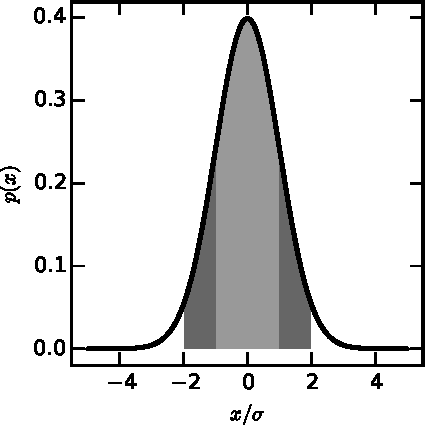
\includegraphics[width=\linewidth]{sigma}
\caption[Proability regions for one and two standard deviations]{The $2\sigma$ (dark gray) and $1\sigma$ (light gray) probability regions, comprising 95\% and 68\% probability, respectively.}
\label{f.sigma}
\end{marginfigure}


\section{Measurements with random fluctuations}

Taking a measurement is not a simple affair.  Suppose, for example, we want to measure the brightness of a star.  First, we do not directly measure the brightness; what happens instead is that the light from the star is focused on a charge-coupled device (CCD)---a semiconductor chip---that converts the photons into electric charge.  The charge is read out from a chip, and we relate that charge to the flux of light incident on the chip.  Now, the power supply to the CCD is not perfect but has some fluctuations in voltage.  There is turbulence in the atmosphere that refracts the starlight. The telescope is a big mechanical device that vibrates. And so on. If we take a set of measurements of some quantity, we will have a distribution of values; our task is to estimate the most likely value for that quantity given the measured values.

It is plausible that each of these fluctuations produces an upward or downward error in our measurement, and the size of each fluctuation varies randomly.  We can therefore think of our measurement as being like a random walk: each source of variation contributes ``one step'', and the end result is that the value $x$ that we measure has a probability to lie in $(x,x+\dif x)$ of
\[ p(x)\,\dif x = \frac{1}{\sqrt{2\pi}\sigma}\exp\left[-\frac{(x-\mu)^{2}}{2\sigma^{2}}\right]\,\dif x. \]
In this case $\mu$ is the ``true'' value of the signal, which we don't know \emph{a priori}.  We also don't know beforehand the value of $\sigma$, which indicates the precision of our measurement.

\newthought{Suppose we make $N$ measurements with values $x_{i}, i=1,\ldots,N$.}  What is the best estimate of $\mu$ and $\sigma$?  Intuitively we expect that these should be
\marginnote{We use $\expect(\mu)$ to mean, ``The expected value of $\mu$'', and likewise for $\expect(\sigma)$.}
\[
	\expect(\mu) = \frac{1}{N}\sum x_{i}\quad\textrm{and}\quad\expect(\sigma) = \sqrt{\frac{1}{N}\sum\left(x_{i}-\bar{x}\right)^{2}},
\]
respectively. To put our expectations on a firmer footing, we note that since the probability to measure a value $x$ is $\prob(x)$ and the $N$ measurements $x_{1}, x_{2}, \ldots, x_{N}$ are independent, the  probability that we measured the set $\{x_{i}\}_{i=1,\ldots,N}$ is
\marginnote{%
	The symbol $\prod$ indicates a product,
	\[ \prod_{i=1}^{N} a_{i} \equiv a_{1}\times a_{2}\times\ldots\times a_{N}. \]
}
\begin{eqnarray*}
	\prob\left(\left\{x_{i}\right\}_{i=1,\ldots,N}\right) &=& \prob(x_{1})\prob(x_{2})\times\ldots\times\prob(x_{N})\\	
	&=& \prod_{i=1}^{N}\frac{1}{\sqrt{2\pi}\sigma}\exp\left[-\frac{(x_{i}-\mu)^{2}}{2\sigma^{2}}\right]\,\dif x_{i}\\
	&=& \left(2\pi\right)^{-N/2}\sigma^{-N}\exp\left[-\frac{1}{2\sigma^{2}}\sum_{i=1}^{N}(x_{i}-\mu)^{2}\right]\,\dif x_{1}\ldots\dif x_{N}.
\end{eqnarray*}
In the absence of additional information, our best guess for $\mu$ and $\sigma$ is to pick values that maximize the probability of our measurements.  To find $\mu$, for example, we take the derivative of $\prob\left(\left\{x_{i}\right\}_{i=1,\ldots,N}\right)$ with respect to $\mu$ and set it to zero to find the maximum,
\marginnote{%
Recall that
\[ \DDx{\exp[f(x)]} = \exp[f(x)] \times \DDx{f}. \]
}
\begin{eqnarray*}
	0 = \dd{}{\mu}\prob\left(\left\{x_{i}\right\}_{i=1,\ldots,N}\right) &=& \prob\left(\left\{x_{i}\right\}_{i=1,\ldots,N}\right)\times\left[\frac{1}{\sigma^{2}}\sum_{i=1}^{N}(x_{i}-\mu)\right]\\
	&=& \prob\left(\left\{x_{i}\right\}_{i=1,\ldots,N}\right)\frac{1}{\sigma^{2}}\times
		\left[\left(\sum_{i=1}^{N}x_{i}\right) - N\mu\right].
\end{eqnarray*}
For this derivative to vanish, the quantity in $\left[\,\right]$ must vanish.
We therefore find that the value of $\mu$ which maximizes the probability that we made this set of measurements to be
\begin{equation}
	\expect(\mu) = \frac{1}{N}\sum_{i=1}^{N}x_{i} \equiv \bar{x}.
\end{equation}
\marginnote{You may notice that $\expect(\sigma)$ depends on $\mu$, which we don't know, but must rather estimate as $\bar{x}$.  If one uses $\bar{x}$ as an \emph{estimate} for $\mu$, then one has to make the uncertainty a bit larger,
\[ \expect(\sigma) = \left[\frac{1}{N-1}\sum_{i=1}^{N}\left(x_{i}-\bar{x}\right)^{2}\right]^{1/2}. \]
To quote \citet{Press2007Numerical-Recip}, ``if the difference between $N$ and $N-1$ [in the formula for $\expect(\sigma)$] ever matters to you, then you are probably up to no good.''
}
\begin{exercisebox}[Expectation value of standard deviation]
Show that
\[
 \expect(\sigma) = \left[\frac{1}{N}\sum_{i=1}^{N}\left(x_{i}-\mu\right)^{2}\right]^{1/2}.
\]
\end{exercisebox}

\begin{quote}
\notebook\ The notebook \texttt{distribution.ipynb} explores further how one assesses the \emph{quality} of these estimates of the mean and standard deviation from a set of measurements. This is followed by \texttt{FittingData.ipynb}, which looks at how one \emph{tests} how well a set of measurements conforms to a hypothesis.
\end{quote}

\newthought{We often want to know the probability distribution for a function of several random variables.}  For example, we might measure the volume of a block as $V=L\times W\times H$, where $L$, $W$, and $H$ are the measured length, width, and height, respectively, and each has an associated uncertainty $\sigma_L$, $\sigma_W$, and $\sigma_H$. What is the resulting uncertainty in $V$?

To make this general, suppose $f(\{x_i\})$ is a function of the $N$ independent random variables $x_1,x_2,\ldots,x_N$.
If the relative values of the uncertainties are small, that is $\sigma_i/x_i \ll 1$, then we can expand $f$ about the values $x_i = \mu_i$:
\begin{equation}
	f\left(\{x_i\}\right) \approx f\left(\{\mu_i\}\right) + \sum_{i=1}^{N} \left.\dd{f}{x_{i}}\right|_{x_{i}=\mu_{i}} 
		\left(x_{i}-\mu_{i}\right).
\end{equation}
To find the width of our distribution, we will compute
\[ \sigma_{f}^{2} = \langle\left(f-\langle f\rangle\right)^{2}\rangle \]
In the limit of a large number of measurements, we assume that $\langle f\rangle \approx f(\left\{\mu_{i}\right\})$; then
\[
	f-\langle f\rangle \approx \sum_{i=1}^{N}\left.\dd{f}{x_{i}}\right|_{x=\mu_{i}} (x_{i}-\mu_{i})
\]
and the width $\sigma_{f}^{2}$ is
\[
	\left\langle (f-\langle f\rangle)^{2}\right\rangle = \left\langle \left[\sum_{i=1}^{N} 
		\left.\dd{f}{x_{i}}\right|_{x=\mu_{i}} (x_{i}-\mu_{i})\right]^{2}\right\rangle .
\]
We then expand the square of the term in $\left[\,\right]$ to obtain
\begin{eqnarray}
	\lefteqn{\left\langle\sum_{i=1}^{N}\left(\dd{f}{x_{i}}\right)^{2}
			\left(x_{i}-\mu_{i}\right)^{2}
		+ \sum_{i\neq j} \dd{f}{x_{i}}\dd{f}{x_{j}} 
			\left(x_{i}-\mu_{i}\right)\left(x_{j}-\mu_{j}\right)\right\rangle} \nonumber\\
	&=& \sum_{i=1}^{N} \left(\dd{f}{x_{i}}\right)^{2}
		\left\langle\left(x_{i}-\mu_{i}\right)^{2}\right\rangle \nonumber\\
	 && + \sum_{i\neq j} \dd{f}{x_{i}}\dd{f}{x_{j}} 
			\left\langle\left(x_{i}-\mu_{i}\right)\left(x_{j}-\mu_{j}\right)\right\rangle .
\label{e.width-expanded}
\end{eqnarray}
Now, if the variables $x_{i}$ are completely independent, then
\[ \left\langle\left(x_{i}-\mu_{i}\right)\left(x_{j}-\mu_{j}\right)\right\rangle
	= 	\left\langle\left(x_{i}-\mu_{i}\right)\right\rangle
		\left\langle\left(x_{j}-\mu_{j}\right)\right\rangle = 0
\]
and therefore
\begin{equation}\label{e.propagation-uncertainities}
\sigma_{f}^{2} = \langle\left(f-\langle f\rangle\right)^{2}\rangle 
	= \sum_{i=1}^{N} \left(\dd{f}{x_{i}}\right)^{2} \sigma_{i}^{2}
\end{equation}
This is an important result: it tells us how to propagate uncertainties.  To go back to our example, suppose we measure the length $L$, width $W$, and height $H$ of a block with associated uncertainties $\sigma_L$, $\sigma_W$, and $\sigma_H$.
The uncertainty in our volume is then\marginnote{%
We use the relation $\partial V/\partial L = W\times H = V/L$, and so on for the derivatives w.r.t.\ $W$ and $H$.}
\begin{equation}\label{e.uncertainty-volume}
	\sigma_{V}^{2} = \left(\frac{V}{L}\right)^{2}\sigma_{L}^{2}
		+ \left(\frac{V}{W}\right)^{2}\sigma_{W}^{2}
		+ \left(\frac{V}{H}\right)^{2}\sigma_{H}^{2}
\end{equation}
or
\[ \frac{\sigma_{V}}{V} = 
	\sqrt{\left(\frac{\sigma_{L}}{L}\right)^{2}
	+ \left(\frac{\sigma_{W}}{W}\right)^{2}
	+ \left(\frac{\sigma_{H}}{H}\right)^{2} }.
\]
Using equation~(\ref{e.propagation-uncertainities}) we can derive general rules for propagating uncertainties.

\begin{exercisebox}[Propagation of uncertainties]
Demonstrate the following rules for propagating uncertainties. In these equations, $x$ and $y$ are independent random variables, and $a$ and $b$ are constants.
\begin{enumerate}
\item For $f = ax + by$, show that 
\[ \sigma_{f} = \sqrt{ a^{2}\sigma_{x}^{2} + b^{2}\sigma_{y}^{2}}. \]
\item For $f = x^{a}y^{b}$, show that
\[ 
	\frac{\sigma_{f}}{f} = \sqrt{ a^{2}\left(\frac{\sigma_{x}}{x}\right)^{2} 
		+ b^{2}\left(\frac{\sigma_{y}}{y}\right)^{2} }.
\]
\end{enumerate}
\end{exercisebox}

\begin{exercisebox}[Examples of propagation of uncertainties]
\begin{enumerate}
\item Given $g$ and $t$ with uncertainties $\sigma_{g}$ and $\sigma_{t}$, find $\sigma_{s}$ with
\[	s = \frac{1}{2}gt^{2}.	\]
\item Given $V$ and $\varpi$ with uncertainties $\sigma_{V}$ and $\sigma_{\varpi}$, find $\sigma_{M}$ with
\[	M = V + 5 - 5\log\left(\frac{1}{\varpi}\right).	\]
\item Given $A$ and $P$ with uncertainties $\sigma_{A}$ and $\sigma_{P}$, find $\sigma_{z}$ with
\[	z = A\sin\left(\frac{2\pi t}{P}\right).	\]
\end{enumerate}
\end{exercisebox}

\newthought{An interesting special case of equation~(\ref{e.propagation-uncertainities})} is when we make a number of repeated measurements $x_{i}, i=1,\ldots,N$ and we wish to compute their average
\[ \bar{x} = \frac{1}{N}\sum_{i=1}^{N}x_{i} . \]
Since each measurement has the same uncertainty $\sigma$, the uncertainty in our average---the \newterm{error in the mean}---is
\begin{equation}\label{e.error-mean}
 \sigma_{\bar{x}} = \frac{1}{N}\sqrt{\sum_{i=1}^{N}\sigma^{2}}
 	= \frac{1}{N}\sqrt{N\sigma^{2}}
  = \frac{\sigma}{\sqrt{N}}.
\end{equation}
\emph{By making many repeated measurements, the uncertainty in the mean due to random fluctuations can be made much less than the uncertainty of any single measurement.}

\begin{exercisebox}[Illustration of error in the mean]
Suppose during an election ten independent polls each show that candidate A is leading with $50.3\%$ of the vote. Since the margin of error---the uncertainty---in each poll is $\pm 1\%$, the news anchor reports that the election is a dead heat.  Is this correct?  What is the probability of candidate A receiving more than $50\%$ of the vote, assuming that the errors in the polls follow a normal (Gaussian) distribution with $\sigma = 1\%$?
\end{exercisebox}

\newthought{Now we can generalize our discussion} to the case of making $N$ measurements, but with each measurement $x_{i}$ having a different uncertainty $\sigma_{i}$.  What is our estimate for $\mu$, and what is our estimate of $\sigma_{\mu}$, the uncertainty in $\mu$?  To answer, we go back to finding the value of $\mu$ that maximizes the probability of us obtaining a sequence of measurements $\{x_{i}\}_{i=1,\ldots,N}$,
\begin{eqnarray*}
	0 = \dd{}{\mu}\prob\left(\left\{x_{i}\right\}_{i=1,\ldots,N}\right) &=& 
		\dd{}{\mu}\prob(x_{1})\prob(x_{2})\ldots\prob(x_{N})\\
	&=&	\prob\left(\left\{x_{i}\right\}_{i=1,\ldots,N}\right) 
		\times \sum_{i=1}^{N}\frac{x_{i}-\mu}{\sigma_{i}^{2}}
\end{eqnarray*}
Hence the expected (most likely) value of $\mu$ is
\begin{equation}
	\expect(\mu) = \frac{\sum_{i=1}^{N} x_{i}/\sigma_{i}^{2}}{\sum_{i=1}^{N} 1/\sigma_{i}^{2}}.
\end{equation}
Note that in the limit $\sigma_{i}\to \sigma$, then $\expect(\mu)\to \sum x_{i}/N$, as it should.

We can compute the uncertainty in $\expect(\mu)$ 
from equation~(\ref{e.propagation-uncertainities}),
\begin{equation}
	\sigma_{\mu}^{2} = \sum_{i=1}^{N} \left(\dd{\mu}{x_{i}}\right)^{2} \sigma_{i}^{2} = \frac{\sum_{i=1}^{N}1/\sigma_{i}^{2}}{\left(\sum_{i=1}^{N}1/\sigma_{i}^{2}\right)^{2}} = \frac{1}{\sum_{i=1}^{N}1/\sigma_{i}^{2}}.
\end{equation}
As before, in the limit $\sigma_{i}\to\sigma$, $\sigma_{\mu}\to\sigma/\sqrt{N}$.

